\msection{Offensive Diversification: Malware evasion}


The primary black-hat usage of WebAssembly is cryptojacking \cite{10.1145/3488932.3517411}. 
Such WebAssembly code mines cryptocurrencies on users' browsers for the benefit of malicious actors and without the consent of the users \cite{ 10.1145/3339252.3339261}.
The main reason for this phenomenon is that the core foundation of cryptojacking is: the faster, the better.
In this context, WebAssembly, a binary instruction format designed to be portable and fast, is a feasible technology for implementing and distributing cryptojacking over the web.
A Kaspersky report about the state of cryptojacking in the first three quarters of 2022 confirms the steady growth in the usage of cryptominers \cite{kasperksy}.
The report shows that Monero \cite{monero} is the most used cryptocurrency for cryptomining in the browser.
Attackers might hide WebAssembly cryptominers \cite{9566204} in multiple locations inside web applications.

Antivirus and browsers provide support for detecting cryptojacking. 
For example, the Firefox browser supports the detection of cryptomining by using deny lists \cite{firefoxcrypto}.
The academic community also provides related work on detecting or preventing WebAssembly cryptojacking \cite{SEISMIC, minos, coinspy, MineThrotle, outgard,9286112}.
Yet, it is known that black-hats can use evasion techniques to bypass detection.
Only the previous work of Bhansali \etal \cite{10.1145/3507657.3528560} investigates the possibility of WebAssembly cryptojacking to evade detection techniques. This is a crucial motivation for our work, one of the first to study WebAssembly malware evasion.


\todo{Present the SOTA of malware evasion. The assumption on lack of diversity in the malware detectors, not that much, check authors.}
\todo{Then present the threat model image here}


\msubsection{Threat model and objective}



In this paper, we design, implement and evaluate a  full-fledged evasion pipeline for WebAssembly.
Concretely, we use wasm-mutate as a diversifier \cite{wasm-mutate}, which implements 135 possible bytecode transformations, grouped into three categories: peephole operator, module structure, and control flow.
We demonstrate the effectiveness of our evasion technique against two cryptojacking detectors: VirusTotal, a general detection tool that comprises 60 antiviruses and, MINOS \cite{minos}, a WebAssembly-specific detector.



\todo{Detail the threat model and make a clear statement of the objective of this use case.}

\begin{figure}
    \centering
    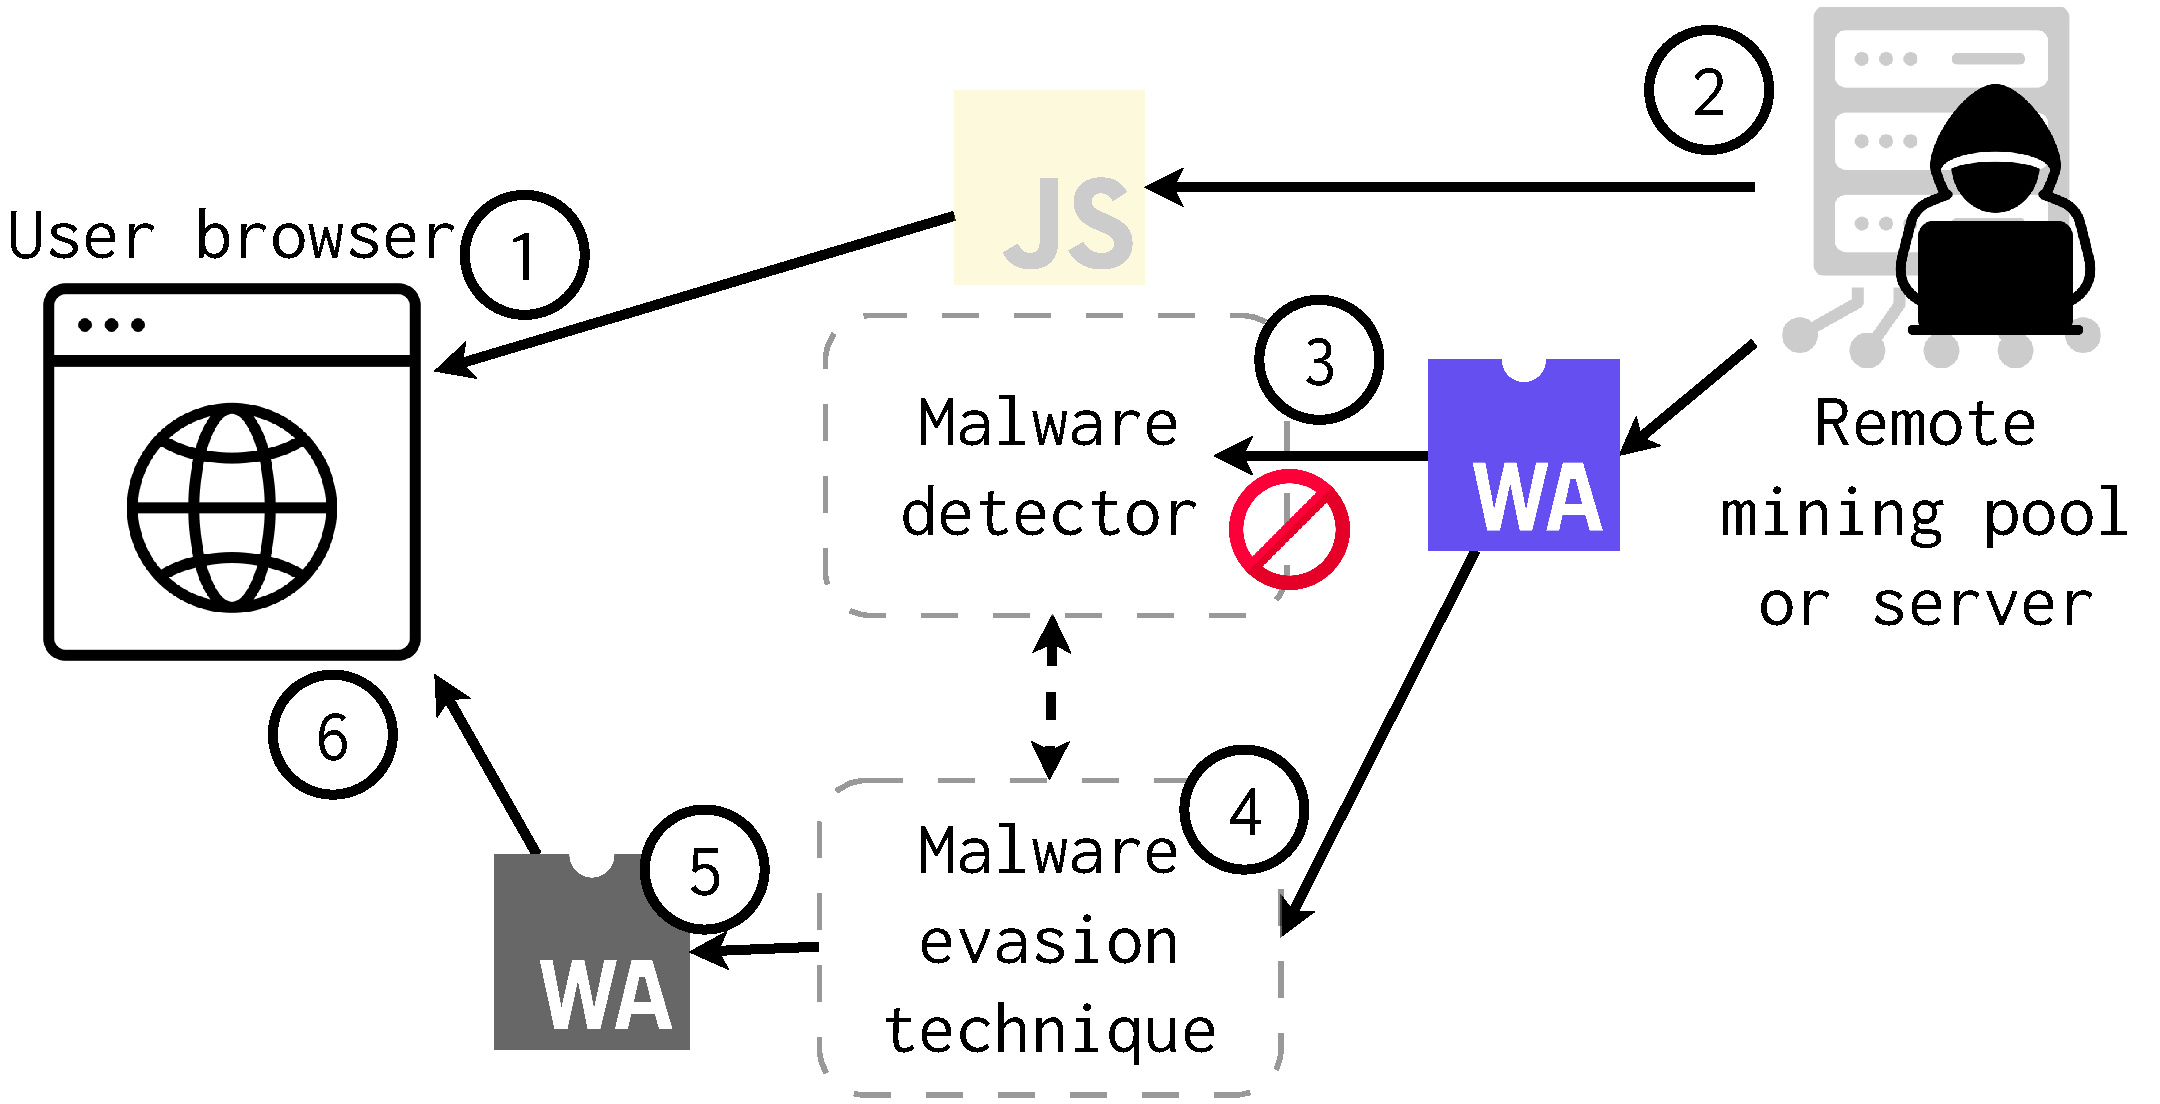
\includegraphics[width=0.8\linewidth]{figures/threat_model.pdf}
    \caption{Taken from \cite{EVASION}}
    \label{fig:threat_model}
\end{figure}

Test and evade the resilience of \Wasm malware detectors mentioned in \autoref{background:wasm:ecosystems}.


\msubsection{Approach}


We evaluate our proposed evasion technique on 33 cryptojacking malware that we curated from the 8643 binaries of the wasmbench dataset \cite{Hilbig2021AnES}, to our knowledge, the most exhaustive collection of real-world WebAssembly binaries.
We experiment with the 33 binaries marked as potentially dangerous by at least one antivirus vendor of VirusTotal.
We empirically demonstrate that evasion is possible for all of these 33 real-world WebAssembly cryptojacking malware while using a WebAssembly-specific detector. 
Remarkably, we find 30 cryptominers for which our technique successfully generates variants that evade VirusTotal.
Our set of malware includes 6 cryptojacking programs that are fully reproducible in a controlled environment. 
With them, we assess that our evasion method does not affect malware correctness and generates fully functional malware variants with minimal overhead.

Our work provides evidence that the malware detection community has opportunities to strengthen the automatic detection of cryptojacking WebAssembly malware. 
The results of this work are actionable, as we provide quantitative evidence on specific malware transformations on which detection methods can focus.

\todo{Mention the uncontrolled and controlled diversification. What are the difference between them. Make a statement about that obfuscation is a face of diversificaation. Specifically, controlled diversification.}

%\lipsum[1]

\todo{We use wasm-mutate}
\todo{How do we use it?}
\todo{Controlled and uncontrolled diversification.}

%\lipsum[1]

%\lipsum[1]

\msubsection{Results}


\begin{tcolorbox}[title=Contribution paper,boxrule=1pt,arc=.2em,boxsep=1.0mm]
    The case discussed in this section is fully detailed in Cabrera-Arteaga \etal "WebAssembly Diversification for Malware Evasion"
    \emph{at Computers \& Security, 2023}
    \url{https://www.sciencedirect.com/science/article/pii/S0167404823002067}. 
\end{tcolorbox}


\emph{Discussion}
In this section we mention some challenges we face during the writing of this work.
We enumerate them in order to enforce the debase and the discussion on the topic.

\emph{Oracle classification moves in time:}
One could expect that the more detectors a binary has, the more iterations are needed to evade them.
However, we have observed that this is not the case for some binaries.
The main reason is that the final labelling of binaries for VirusTotal vendors is not immediate \cite{251586}. 
For example, a VirusTotal vendor could label a binary as benign and change it later to malign after several weeks in a conservative way of acting.
This phenomenon creates a time window in which slightly changed binaries (fewer iterations in our case) could evade the detection of numerous vendors.

\emph{Lack of bigger picture:} A WebAssembly cryptomalware can only exist with its JavaScript complement.
For example, a browser cryptonalware needs to send the calculated hashes to a cryptocurrency service.
This network communication is outside the WebAssembly accesses and needs to be delegated to a JavaScript code.
Besides, other functionalities can be intermixing between JavaScript and WebAssembly and in some cases be completely in one side or the other \cite{romano2022wobfuscator}.
This intermixing between JavaScript and WebAssembly could provide statically different WebAssembly. 
% What we saw
We have observed that, the imports and the memory data of the WebAssembly binaries have a high variability in our original dataset.
The imported functions from JavaScript change from binary to binary.
Their data segments can also differ in content and length.
To completely analyze these cases, the whole JavaScript-WebAssembly program is needed, something only provided in 9/33 cases of our dataset.

\emph{More narrowed fitness function:} We use a simple fitness function, but the MCMC evasion algorithm could have a fitness function as general as wanted.
In our case, we do not use binary metadata, instead we focus on the result from the malware oracle, given that the main goal is to evade this oracle.

\emph{Mitigation: } \todo{TBD, data augmentation, better resilience evaluation ?}


Another interesting thing would be to see if there is difference in the detectors. If some detectors are fooled by some transformations or are more robust, etc.

\todo{Motivate the use case with the following sota}

\wrule{Binary rewriting tools and obfuscators} The landscape for tools that can modify, obfuscate, or enhance \Wasm binaries for various has increased. 
For instance, BREWasm\cite{BREWasm} provides a comprehensive static binary rewriting framework specifically designed for \Wasm. 
Wobfuscator\cite{wobfuscator} takes a different approach, serving as an opportunistic obfuscator for Wasm-JS browser applications. 
Madvex\cite{madvex} focuses on modifying \Wasm binaries to evade malware detection, with its approach being limited to alterations in the code section of a \Wasm binary. 
Additionally, WASMixer\cite{wasmixer} obfuscates WebAssembly binaries, by including memory access encryption, control flow flattening, and the insertion of opaque predicates.


\todo{ The malware evasion paper}
